% !TEX encoding = UTF-8
% !TEX TS-program = pdflatex
% !TEX root = ../tesi.tex

%**************************************************************
\chapter{Introduzione}
\label{cap:introduzione}
%**************************************************************

% Introduzione al contesto applicativo.\\

% \noindent Esempio di utilizzo di un termine nel glossario \\
% \gls{api}. \\

% \noindent Esempio di citazione in linea \\
% \cite{site:agile-manifesto}. \\

% \noindent Esempio di citazione nel pie' di pagina \\
% citazione\footcite{womak:lean-thinking} \\

%**************************************************************
\section{L'azienda}

Sync Lab nasce a Napoli nel 2002 come software house ed è rapidamente cresciuta nel
mercato dell’Information and Comunications Tecnology (ICT). 
\\\\
A seguito di una
maturazione delle competenze tecnologiche, metodologiche ed applicative nel dominio
del software, l’azienda è riuscita rapidamente a trasformarsi in \gls{System Integrator}\glsfirstoccur conquistando 
significative fette di mercato nei settori mobile, videosorveglianza e sicurezza
delle infrastrutture informatiche aziendali. 
\\\\
Attualmente, Sync Lab ha più di 150 clienti
diretti e finali, con un organico aziendale di 300 dipendenti distribuiti tra le 6 sedi
dislocate in tutta Italia.
Sync Lab si pone come obiettivo principale quello di supportare il cliente nella realizzazione, 
messa in opera e governance di soluzione \gls{IT}\glsfirstoccur, sia dal punto di vista tecnologico,
sia nel governo del cambiamento organizzativo.

\begin{figure}[H]
    \centering
    
\includegraphics[height=2.5cm]{logo-synclab}
    \caption{Logo Sync Lab}
\end{figure}

%**************************************************************
\section{Scelta dell'azienda}
Sono venuto a conoscenza dell'azienda Sync Lab grazie al progetto d'ingegneria del
software, dove l'azienda è stata il proponente del mio progetto.
\\\\
Sono venuto a conoscenza del progetto di stage di Sync Lab grazie all'evento stage-it 2022. 
L’evento promosso da Assindustria Venetocentro in collaborazione con l’Università 
di Padova per favorire l’incontro tra aziende con progetti innovativi in ambito \gls{IT} e 
studenti dei corsi di laurea in Informatica, Ingegneria informatica e Statistica.
\\\\


%**************************************************************
\section{Introduzione al progetto}

Lo scopo del progetto di stage consiste nell'effettuare la migrazione di un servizio di
\gls{API}\glsfirstoccur \gls{REST}\glsfirstoccur, lato back-end, realizzato da un precedente studente tirocinante con il framework
Spring, in un servizio di \gls{API} \gls{REST}, lato \gls{back-end}\glsfirstoccur, realizzato con un diverso framework chiamato
NestJS. Il proponente ha deciso di fare la migrazione per effettuare un'analisi comparativa tra le due soluzioni, in
modo da valutarne le caratteristiche e decidere quale dei due meglio si adatta alle esigenze
del progetto.
\\\\
Il progetto consiste nella realizzazione di una webapp che si occupa di gestire un sistema
di controllo parcheggi auto. Il sistema va ad interrogare una base di dati contenente
l'informazione inerente allo stato di alcuni sensori di parcheggio, fornendo la visualizzazione
dei posti liberi/occupati all'interno di una mappa.
\\\\
L'idea del progetto nasce per agevolare un utente che vuole usufruire di un posto auto all'interno di 
un parcheggio e non vuole perdere tempo in cerca di un posto libero e nemmeno uscire di casa se i posti auto
sono tutti occupati; infatti la webapp oltre a mostrare su una mappa le piazzole libere o occupate, segnala 
anche la disponibilità di posti auto in un parcheggio e il tutto viene fatto in tempo reale.
\\\\
E' prevista poi la realizzazione di una sezione dedicata ai manutentori, in modo che possano monitorare
in tempo reale lo stato dei sensori, facilitando quindi il processo di manutenzione.
\\\\
Il progetto è formato da una parte di \gls{front-end}\glsfirstoccur, realizzata con il framework Angular e una 
parte di \gls{back-end} che consiste di un servizio di \gls{API} \gls{REST}, realizzato in due versioni: una 
con il framework Spring e una con il framework NestJS.
\\
Questo progetto di stage riguarda la parte di \gls{back-end}, un altro mio collega stagista si sta occupando
della parte di \gls{front-end}.
\clearpage
\begin{figure}[H]
    \centering
    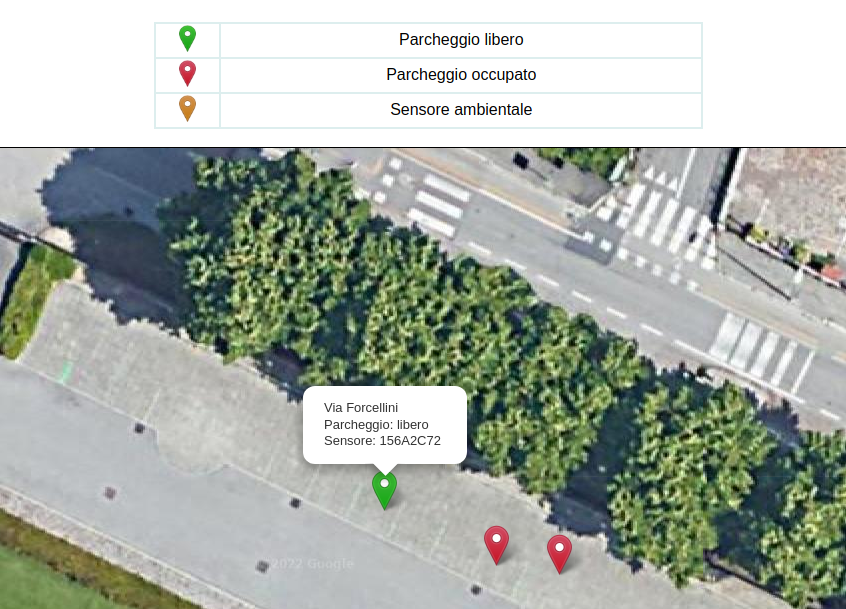
\includegraphics[height=9cm]{front-end-smart-parking}
    \caption{Front-end Smart Parking}
\end{figure}

%**************************************************************
\section{Problematiche riscontrate}
Durante lo svolgimento del progetto si sono presentate alcune criticità, alcune dovute alla mancanza
di conoscenza delle tecnologie da utilizzare. 
\\
Le problematiche riscontrate:

\begin{itemize}
    \item architettura a microservizi: avevo solo una conoscenza basilare
          della tecnologia, grazie al corso d'ingegneria del software ma non
          sufficiente per fare un'analisi di migrazione futura del progetto, in un progetto con 
          architettura a microservizi;
    \item framework Spring: la conoscenza di questo framework era completamente assente
        ed era importante conoscerlo per poter comprendere con chiarezza il software esistente,
        di cui doveva essere effettuata la migrazione;
    \item framework Node.js e NestJS: la conoscenza di questi due framework era completamente
        assente ed era di fondamentale importanza conoscerli per poter implementare il servizio
        di \gls{API} \gls{REST}, lato back-end, richiesto;
    \item la quantità di \gls{API} \gls{REST} da migrare era troppo elevata per il tempo a disposizione;
    \item il modello della base dati ha dovuto subire adeguamenti rispetto alla prima versione
        per rappresentare nel modo migliore lo scenario funzionale.
\end{itemize}

%**************************************************************
\section{Soluzione scelta}

E' stato scelto di sviluppare il progetto con un architettura di tipo layered architecture. Questo è uno
degli stili architetturali più utilizzati quando si sviluppa un software monolitico. L'idea dietro a 
questa architettura è che i moduli con funzionalità simili sono organizzati in livelli
orizzontali. Quindi ogni livello svolge uno specifico ruolo nell'applicazione.
\\\\
La layered architecture astrae la visione del sistema nel suo insieme, fornendo dettagli 
sufficienti per comprendere ruoli e le responsabilità dei singoli livelli e le relazioni
che intercorrono tra loro.
\\\\
La motivazione che ha portato alla scelta di questo stile architetturale è un'analisi fatta,
che ha rivelato, che la layered si adatta molto bene al servizio di \gls{API} \gls{REST} che
si vuole andare a realizzare. Inoltre molti framework per lo sviluppo di applicativi \gls{back-end} si basano su questo tipo di architettura, tra cui
Spring e NestJS, che sono fondati sul pattern controller-service-repository. Un pattern
che sfrutta la layered architecture, creando tre diversi livelli di astrazione: 
\begin{itemize}
    \item controller: è il livello più alto ed è l'unico responsabile dell'esposizione delle
        funzionalità, in modo che possano essere consumate da entità esterne;
    \item service: livello centrale, gestisce tutta la business logic;
    \item repository: livello più basso, è responsabile di salvare e recuperare i dati da un
        sistema di persistenza, come un database.
\end{itemize}
\clearpage
\leavevmode\newline
Quest'architettura viene utilizzata per effettuare una buona separazione delle responsabilità.
\\
L'architettura usata da Spring e NestJS è proprio la stessa che si è deciso di usare nell'analisi progettuale fatta 
 e quindi questi due framework sono stati scelti per realizzare
la parte di \gls{back-end} del progetto.
\leavevmode\newline
\begin{figure}[H]
    \centering
    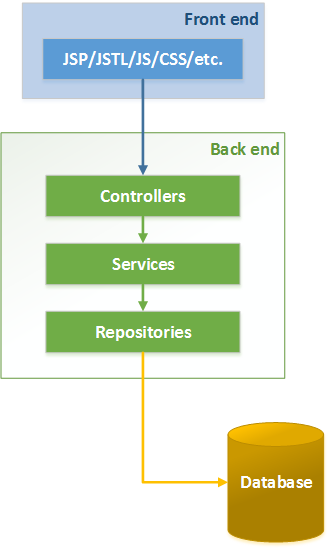
\includegraphics[height=9cm]{controller-service-repository-pattern}
    \caption{Controller-service-repository pattern}
\end{figure}
\leavevmode\newline
Non è prevista la creazione di un sistema di autenticazione per l'uso delle \gls{API} \gls{REST}, in quanto 
un altro studente tirocinante si sta occupando della creazione di questa parte.

%**************************************************************
\section{Descrizione del prodotto ottenuto}

Al momento è disponibile un \gls{back-end} contenente le \gls{API} \gls{REST} sviluppate in NestJS, utilizzabile in produzione,
anche se non potendo migrare l'intero set di \gls{API} \gls{REST} disponibili nella soluzione realizzata in Spring, come preventivato,
sono state sviluppate tutte le \gls{API} \gls{REST} più importanti per effettuare le operazioni \gls{CRUD}\glsfirstoccur più
comuni.
\\\\
Le \gls{API} \gls{REST} espongono un'interfaccia compatibile con quello che ormai è uno standard per la
comunicazione con servizi di tipo \gls{REST}. Ovvero per comunicare con le \gls{API} \gls{REST} bisogna fare
delle richieste \gls{HTTP}\glsfirstoccur a degli specifici \gls{endpoint} con i seguenti metodi \gls{HTTP}:
\begin{itemize}
    \item GET: per ottenere delle risorse dal servizio \gls{REST};
    \item POST: per creare una nuova risorsa nel servizio \gls{REST};
    \item PUT: per modificare una risorsa nel servizio \gls{REST};
    \item DELETE: per eliminare una risorsa dal servizio \gls{REST}.
\end{itemize}
\leavevmode\newline
E' presente poi, nel \gls{back-end}, un servizio schedulato che ogni due minuti in maniera autonoma va a fare il polling
da un file \gls{XML}\glsfirstoccur online, contenente gli stati aggiornati dei sensori. Questo servizio registra poi 
le variazioni, rispetto
al polling precedente, nel servizio di persistenza.
\\\\
Il file \gls{XML} viene scritto e gestito dai produttori dei sensori di parcheggio, quindi non è compito di questo 
progetto gestirne il funzionamento. Il funzionamento di questo file \gls{XML} è comunque abbastanza banale,
in quanto ad ogni variazione di stato il sensore di parcheggio va semplicemente ad aggiornare 
il record a lui associato
all'interno del file.
\\\\

%**************************************************************
\section{Tecnologie utilizzate}

\textbf{Git}
\\\\
E' uno degli strumenti di controllo di versionamento più utilizzati. Facilita la collaborazione
tra gli sviluppatori nella realizzazione di un progetto e permette con semplicità di spostarsi
tra varie versioni del software realizzate. Nel progetto è stato utilizzato con il workflow
Gitflow.
\\\\\\
\textbf{Visual Studio Code}
\\\\
E' un editor di codice sorgente sviluppato da Microsoft che aiuta lo sviluppatore durante la fase
di sviluppo del codice in quanto evidenzia le parole chiave, segnala errori di scrittura, suggerisce
snippet di codice. Possiede una grande libreria di estensioni facilmente installabili per renderlo
compatibile con praticamente qualsiasi linguaggio di programmazione.
\\\\\\
\textbf{Postman}
\\\\
E' un'applicazione che viene utilizzata solitamente per testare \gls{API}. E' un client \gls{HTTP} che testa richieste
\gls{HTTP} utilizzando una \gls{GUI}\glsfirstoccur, attraverso la quale otteniamo diversi tipi di risposta in base alle \gls{API} che 
andiamo ad interrogare.
\\\\\\
\clearpage
\leavevmode\newline
\textbf{Stoplight}
\\\\
E' una piattaforma per progettare \gls{API}. Grazie a questo strumento è possibile documentare in maniera rigorosa
e su uno spazio in cloud un set di \gls{API}. La piattaforma permette di specificare varie informazioni per ogni
\gls{API}, tra cui \gls{endpoint}\glsfirstoccur, parametri in ingresso attesi, possibili risposte con status code associato. Questo
strumento è molto utile per gli sviluppatori \gls{front-end} che devono chiamare le \gls{API} di un servizio
\gls{back-end}, soprattutto grazie alla funzionalità che permette di generare il \gls{mock}\glsfirstoccur della risposta di un'\gls{API}, 
permettendo allo sviluppatore di effettuare le chiamate al \gls{back-end} anche senza che questo sia stato ancora realizzato.
\\\\\\
\textbf{TypeScript}
\\\\
E' un superset di JavaScript, che aggiunge tipi, classi, interfacce e moduli opzionali al JavaScript 
tradizionale. Si tratta sostanzialmente di una estensione di JavaScript.
TypeScript è un linguaggio tipizzato, ovvero aggiunge definizioni di tipo statico: i tipi consentono di 
descrivere la forma di un oggetto, documentandolo meglio e consentendo a TypeScript di verificare che 
il codice funzioni correttamente.
\\\\\\
\textbf{Node.js}
\\\\
E' un runtime system open source per eseguire applicazioni scritte in JavaScript, permettendoci di utilizzare questo 
linguaggio, tipicamente utilizzato nella client-side, anche per la scrittura di applicazioni server-side.
La piattaforma è basata sul JavaScript Engine V8, che è il runtime di Google utilizzato anche da Chrome e 
disponibile sulle principali piattaforme, anche se maggiormente performante su sistemi operativi UNIX-like.
\\\\\\
\textbf{NestJS}
\\\\
E' un framework per la creazione di applicazioni lato server Node.js efficienti e scalabili. 
Utilizza JavaScript ma è costruito con e supporta completamente TypeScript. Aggiunge un livello di astrazione
al framework Express, che a sua volta aggiunge astrazione al framework Node.js. Di conseguenza NestJS 
utilizza Node.js per eseguire il codice JavaScript generato dalla compilazione del codice TypeScript.
\\\\\\
\textbf{Spring}
\\\\
Spring è un framework leggero, basato su Java. Questo framework integra soluzioni a vari problemi tecnici
che si presentano con alta frequenza durante lo sviluppo software. Spring si basa su due design pattern
fondamentali che sono l'Inversion of Control e Dependency Injection.
\\\\\\
\clearpage
\leavevmode\newline
\textbf{PostgreSQL}
\\\\
Chiamato anche Postgres, è un sistema di database relazionale a oggetti (ORDBMS), open source e 
gratuito.
Le principali caratteristiche di Postgres sono affidabilità, integrità dei dati, funzionalità ed estensibilità, 
oltre alla propria community open source che gestisce, aggiorna e sviluppa soluzioni performanti e innovative.
\\\\\\
\textbf{Jest}
\\\\
Jest è un framework di unit test sviluppato da Facebook. Focalizzato sulla semplicità, è utilizzabile in qualsiasi
progetto JavaScript. E'uno dei framework di test JavaScript più popolare in questi giorni e la scelta di default 
per alcuni framework come NestJS e React.
\\\\\\
\textbf{Winston}
\\\\
Winston è una delle libreria più famose per effettuare il logging su applicazioni Node.js. Permette di effettuare il logging
su più livelli di informazione, formattare il logging in modo predefinito, scegliere la destinazione di output del log e molte 
altre opzioni.
\\\\\\
\textbf{Npm}
\\\\
E' uno dei gestori di pacchetti per il linguaggio JavaScript più popolare. E' il gestore di pacchetti predefinito 
per Node.js.

%**************************************************************
\section{Organizzazione del testo}

\begin{description}
    \item[{\hyperref[cap:analisi-requisiti]{Il secondo capitolo}}] descrive l'analisi dei requisiti.
    
    \item[{\hyperref[cap:progettazione]{Il terzo capitolo}}] approfondisce la fase di progettazione.
    
    \item[{\hyperref[cap:ristrutturazione-database]{Il quarto capitolo}}] descrive la fase di ristrutturazione del database.
    
    \item[{\hyperref[cap:verifica-e-validazione]{Il quinto capitolo}}] descrive la fase di verifica e validazione.
    
    \item[{\hyperref[cap:analisi-comparativa]{Il sesto capitolo}}] approfondisce l'analisi comparativa tra la soluzione in Spring e quella in NestJS.
    
    \item[{\hyperref[cap:conclusioni]{Il settimo capitolo}}] presenta le conclusioni finali sul progetto e sull'esperienza di stage.
\end{description}

Riguardo la stesura del testo, relativamente al documento sono state adottate le seguenti convenzioni tipografiche:
\begin{itemize}
	\item gli acronimi, le abbreviazioni e i termini ambigui o di uso non comune menzionati vengono definiti nel glossario, situato alla fine del presente documento;
	\item per la prima occorrenza dei termini riportati nel glossario viene utilizzata la seguente nomenclatura: \emph{parola}\glsfirstoccur.
\end{itemize}